\section{Lektion 06-02-2018}

\begin{enumerate}
	\item ADC Quantization
	\item Coefficient- and Product-Quantization
	\item Overflow/Underflow and Coefficient Scaling
	\item Notch- and Peak-filters as example
\end{enumerate}

\begin{mdframed}[style=exampledefault]
\begin{itemize}
	\item ESP 6.1.1 (only p. 222 - 229)
	\item ESP 6.2.2, 6.2.3 (p. 240 - 243)
	\item ESP 3.4.2 + 3.4,3
\end{itemize}
\end{mdframed}

\subsection{ADC Quantization}

\subsubsection{Dynamic Range and Signal-to-Quantization Noise Ratio}
The dynamic range of a digital signal is defined as the difference between the largest and smallest signal values.
If noise is present in the system, the dynamic range is the difference between the largest signal level and the noise floor.
When performing signal processing, a higher precision ($>$16 bits) is normally preferred to maintain this level of dynamic range.
\begin{itemize}
	\item Dynamic range
	\begin{itemize}
		\item Typical in relation to "\SI{0}{\decibel} full scale"
	\end{itemize}
\end{itemize}
\begin{equation}
dynamic range = 20\log(\frac{max \: signal \: level}{noise \: floor}) [\si{\decibel}]
\end{equation}
\begin{itemize}
	\item SQNR [\si{\decibel}] $\approx 6\cdot n \;\si{\decibel}$ (n = bits precision)
	\begin{itemize}
		\item Signal-to-quantization noise ratio = $20\log(2^n)$
		\item Different wordlengths of ADC's
		\begin{itemize}
			\item 16-bit fixed-point \SI{96}{\decibel}
			\item 24-bit fixed-point \SI{144}{\decibel}
			\item 32-bit fixed-point \SI{192}{\decibel}
		\end{itemize}
	\end{itemize} 
	\item Dynamic [\si{\decibel}] = Peak Level [\si{\decibel}] - Noise Floor [\si{\decibel}]
\end{itemize}

\begin{figure} [H]
	\centering
	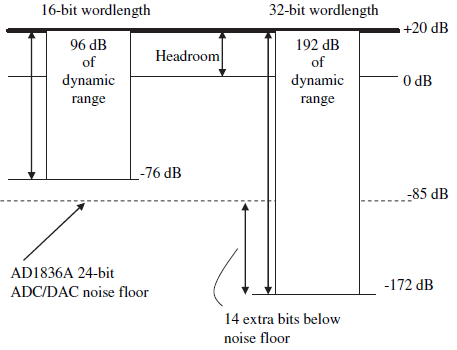
\includegraphics[width=0.85\linewidth]{graphics/9.png}
	\caption{Comparison of different wordlenghts.}
	\label{fig:9}
\end{figure}

\subsubsection{Other sources of quantization errors}
Besides analog-to-digital and digital-to-analog quantization noise, there are other sources of quantization errors in digital systems.

\begin{itemize}
	\item Coefficient quantization
	\item Computational overflow
	\item Quantization error due to truncation and rounding
\end{itemize}

\subsection{Coefficient- and Product-Quantization}
\subsubsection{Coefficient Quantization}
When a digital system is designed for computer simulation, the coefficients are generally represented with floating-point format. 
However, these parameters are usually represented with a finite number of bits in fixed-point processors with a typical wordlength of 16 bits.\\

Coefficient quantization of an IIR filter can affect pole/zero locations, thus altering the frequency response and even the stability of the digital filter.

\begin{itemize}
	\item Only specific values possible for eg. filter coefficients
	\item Only discrete points in pole-zero plane
	\item Deterministic effect – known in advance
\end{itemize}

\subsubsection{Product Quantization}
Truncation or rounding is used after multiplication to store the result back into the memory.\\

In general, the distribution of errors caused by rounding is uniform, resulting in quantization errors with zero mean and variance of $\Delta2/12$. Truncation has a bias mean of $\Delta/2$ and a variance of $\Delta2/12$.
\begin{itemize}
	\item Happens after multiplication (=product) of both fixed- and floating-point numbers (unless	using double number bits)
	\item Can be considered as an added noise term (stochastic)
	\item Limit-cycles may occur
\end{itemize}

\subsection{Quantization and Noise models}
Noise is introduced by multiplications between variables, a noise signal is added e(n).
\subsubsection{Signal Flow Graphs}
\begin{itemize}
	\item Illustration of implementation
	\item Useful for illustration of quantization errors
	\item Different filter-forms available – most try to reduce effects of quantization for fixed-point implementations
\end{itemize}

Assumed that noise \textit{e} is equal distributed
\begin{itemize}
	\item – Product quantization $0 \leq |e| \leq 2^{-(m+1)}$
\end{itemize}

\begin{figure} [H]
	\centering
	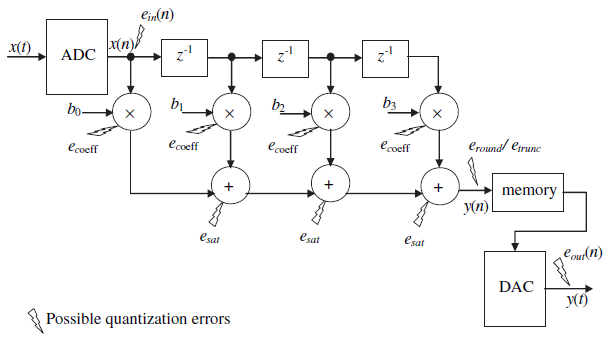
\includegraphics[width=\linewidth]{graphics/10.png}
	\caption{Quantization error sources in a 4-tap FIR filter.}
	\label{fig:10}
\end{figure}

\subsection{Overflow/Underflow and Coefficient Scaling}
Because of the finite memory/register length, the results of arithmetic operations may have too many bits to be fitted into the wordlength of the memory or register.

\begin{itemize}
	\item Causing "random" results or no output
\end{itemize}

A sum of $M \: B$-bit numbers requires $B + \log_2 M$ bits to represent the final result without overflow.
\begin{itemize}
	\item eg. If 256 32-bit numbers	are added, a total of $32 + \log_2 256 =40$ bits are required to save the final result.
\end{itemize}

Overflow/underflow can be avoided with "clever" scaling or, at least, avoided "with a high probability"
\begin{itemize}
	\item Block floating point
	\item Exponent checking
	\item Saturation
	\item Coefficient scaling
\end{itemize}

\subsection{Notch- and Peak-filters}
\begin{itemize}
	\item Can be designed by pole-zero placement
	\item Pole radii and angle determine frequency response
	\item Common buildingblocks	for higher-order IIR
\end{itemize}

\subsubsection{Notch-filter}
A notch filter contains one or more deep notches in its magnitude response. To create a notch at frequency $\omega_0$, a pair of complex-conjugate zeros on
the unit circle at angle $\omega_0$ as $z=e^{\pm j\omega_0}$.\\

\noindent Transfer function of \textbf{FIR} notch filter is  $H(z) = (1-e^{j\omega_0} z^{-1})(1-e^{-j\omega_0} z^{-1})$. This is a filter of order 2 because there are two zeros in the system. Note that a pair of complex-conjugate zeros guarantees that the filter will have real-valued coefficients.\\

The magnitude response has a relatively wide bandwidth, which means that other frequency components around the null are severely attenuated. 
To reduce the bandwidth of the null, we may introduce poles into the system $z_p = r e^{\pm j\phi_0}$. $r$ is the radius, $\phi_0$ is the angle of poles.\\

\noindent Transfer function of \textbf{IIR} notch filter is  $H(z) = \frac{(1-e^{j\omega_0} z^{-1})(1-e^{-j\omega_0} z^{-1})}{(1-r\cdot e^{j\phi_0} z^{-1})(1-r\cdot e^{-j\phi_0} z^{-1})} $. \\

\noindent This is a IIR filter of order 2 because there are two poles in the system.

\begin{figure} [H]
	\centering
	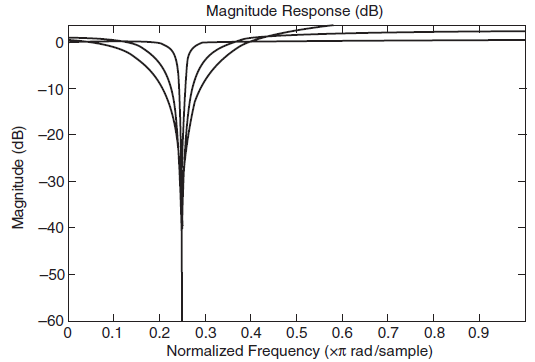
\includegraphics[width=0.85\linewidth]{graphics/11.png}
	\caption{Magnitude responses of notch filter for different values of \textit{r}.}
	\label{fig:11}
\end{figure}

\subsubsection{Peak-filter}
To create a peak (or narrow passband) at frequency $\omega_0$, we may think we can simply follow the example of designing a notch filter by introducing a pair of complex-conjugate poles on the unit circle at angle $\omega_0$.
However the resulting second-order IIR filter will be unstable. To solve this
problem, we have to move the poles slightly inside the unit circle ($r_p < 1$) as $z_p = r_p e^{\pm j \omega_0}$.\\

\noindent Transfer function of IIR peak filter is  $H(z) = \frac{1}{1-r_p e^{j\omega_0} z^{-1})(1- r_p e^{-j\omega_0} z^{-1})}$.\\

\noindent Similar to the second-order IIR notch filter, the magnitude response has a relatively wide bandwidth, which means that other frequency components around the peak will also be amplified. 
To reduce the bandwidth of the peak, we may introduce zeros into the system.\\

\noindent Transfer function of \textbf{IIR} peak filter is  $H(z) = \frac{1-r_z e^{j\omega_0} z^{-1})(1- r_z e^{-j\omega_0} z^{-1})}{1-r_p e^{j\omega_0} z^{-1})(1- r_p e^{-j\omega_0} z^{-1})}$.\\

\noindent The poles must be closer to the unit circle as $r_p > r_z$.

\begin{figure} [H]
	\centering
	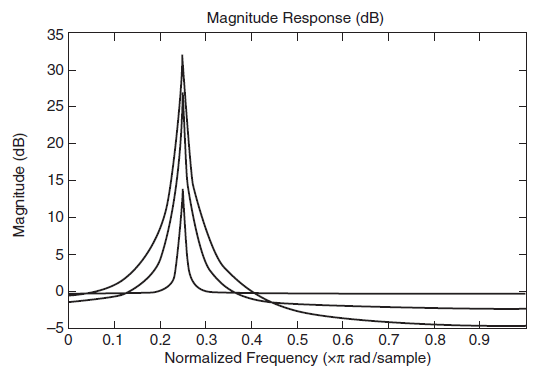
\includegraphics[width=0.85\linewidth]{graphics/12.png}
	\caption{Magnitude responses of peak filter with poles ($r_p = 0.99$) and different radius of zeros.}
	\label{fig:12}
\end{figure}
